% -*- mode: LaTeX/P; fill-column: 80; -*-
% Local Variables:
% eval: (reftex-mode)
% eval: (TeX-PDF-mode)
% End:
% Template for PLoS
% Version 1.0 January 2009

\documentclass[10pt]{article}

% amsmath package, useful for mathematical formulas
\usepackage{amsmath}
% amssymb package, useful for mathematical symbols
\usepackage{amssymb}
\usepackage{tabularx}

% graphicx package, useful for including eps and pdf graphics
% include graphics with the command \includegraphics
\usepackage{graphicx}

% Need to have subfigures
\usepackage{subcaption}
\pdfpagebox5

% cite package, to clean up citations in the main text. Do not remove.
\usepackage{cite}

% Use doublespacing - comment out for single spacing
%\usepackage{setspace} 
%\doublespacing

% Text layout
\topmargin 0.0cm
\oddsidemargin 0.5cm
\evensidemargin 0.5cm
\textwidth 16cm 
\textheight 21cm

% Bold the 'Figure #' in the caption and separate it with a period
% Captions will be left justified
\usepackage[labelfont=bf,labelsep=period,justification=raggedright]{caption}

% Use the PLoS provided bibtex styles
\bibliographystyle{plos2009}

% Remove brackets from numbering in List of References
\makeatletter
\renewcommand{\@biblabel}[1]{\quad#1.}
\makeatother

% Leave date blank
\date{}

\pagestyle{myheadings}
%% ** EDIT HERE **

%% ** EDIT HERE **
%% PLEASE INCLUDE ALL MACROS BELOW
\usepackage[printonlyused]{acronym}
%\usepackage{multicol}

\usepackage{color}
\usepackage{colortbl}
\definecolor{gray9}{gray}{0.9}
\definecolor{gray92}{gray}{0.92}
\definecolor{gray95}{gray}{0.95}
\usepackage[squaren]{SIunits} 
\usepackage{units}
\usepackage{pgfplots}
\usepgfplotslibrary{dateplot}
%\usepgfplotslibrary{statistics}

\newcommand{\pop}{\textit{Populus} }
\newcommand{\note}[1]{\textit{#1}}

\acrodef{3pg}[\textsc{3PG}]{Physiological Principles in Predicting Growth}
\acrodef{BLcond}[\ensuremath{BL_{cond}}]{Canopy Boundary Layer Conductance}
\acrodef{dbh}[\ensuremath{dbh}]{Diameter at Breast Height}
\acrodef{DOB}[\ensuremath{DOB}]{Basal Diameter}
\acrodef{GIS}[\textsc{GIS}]{Geographical Information System}
\acrodef{LAIt}[\ensuremath{LAI_{T}}]{Target Leaf Area Index}
\acrodef{LAI}[\ensuremath{LAI}]{Leaf Area Index}
\acrodef{NPPdef}[\ensuremath{NPP_{def}}]{$NPP$ deficit}
\acrodef{NPPt}[\ensuremath{NPP_{T}}]{$NPP$ if $LAI = LAI_{T}$}
\acrodef{NPP}[\ensuremath{NPP}]{Net Primary Productivity}
\acrodef{RP}[\ensuremath{RP}]{Root Productivity}
\acrodef{Rdp}[\ensuremath{R_{\Delta\%}}]{Root contribution}
\acrodef{SLA}[\ensuremath{SLA}]{Specific Leaf Area}
\acrodef{SRWC}[\textsc{SRWC}]{Short Rotation Woody Crops}
\acrodef{WF}[\ensuremath{W_F}]{Total Foliage Biomass}
\acrodef{WS}[\ensuremath{W_S}]{Total Stem Biomass}
\acrodef{WR}[\ensuremath{W_R}]{Total Root Biomass}
\acrodef{W}[\ensuremath{W}]{Total Plant Biomass}
\acrodef{dRres}[\ensuremath{\Delta R_{res}}]{Residual root contribution}
\acrodef{dW}[\ensuremath{\Delta W}]{Total Monthly Growth}
\acrodef{fAge}[\ensuremath{f_{age}}]{age Growth Limiter}
\acrodef{fR}[\ensuremath{f_R}]{Root conversion efficiency}
\acrodef{fT}[\ensuremath{f_T}]{Temperature growth limiter}
\acrodef{fi}[\ensuremath{f_i}]{Generic growth limiters}
\acrodef{gbsm}[\textsc{GBSM}]{Geospatial Bioenergy Systems Model}
\acrodef{k}[\ensuremath{k}]{Radiation Extinction Coefficient}
\acrodef{lf}[\ensuremath{lf}]{Litterfall}
\acrodef{pRx}[\ensuremath{p_{R\%x}}]{Maximum root \%}
\acrodef{pfs}[\ensuremath{p_{FS}}]{foliage allocation to stem allocation}
\acrodef{VI}[\ensuremath{VI}]{Volume Index}
\acrodef{sps}[\ensuremath{n_{stems}}]{Stems per stump}
\acrodef{cancover}[\ensuremath{CanCover}]{Canopy Coverage}
\acrodef{LA}[\ensuremath{LA}]{Leaf Area per Stem}

%% END MACROS SECTION

\begin{document}

% Title must be 150 characters or less
\begin{flushleft}
{\Large
\textbf{Modeling Poplar Growth as a Short Rotation Woody Crop for Biofuels}
}
% Insert Author names, affiliations and corresponding author email.
\\
Quinn Hart$^{1,\ast}$,
Olga Prelipova$^{2}$,
Justin Merz$^{1}$,
%Peter Tittmann$^{3}$, 
Bryan Jenkins$^{3}$
\\
$^{\textbf{1}}$ Department of Land, Air, and Water, University of California, Davis, USA
$^{\textbf{2}}$ Department of Computer Science, University of California, Davis, USA
%$^{\textbf{3}}$ Department of Forestry, University of California, Berkeley, USA
$^{\textbf{3}}$ Energy Institute, University of California, Davis, USA
\\
%\\textbf{3} Author3 Dept/Program/Center, Institution Name, City, State, Country
$\ast$ E-mail: qjhart@ucdavis.edu
\end{flushleft}

% Please keep the abstract between 250 and 300 words
\section*{Abstract}

\acp{SRWC} have been proposed in an number of studies as a good
potential feedstock for a cellulosic derived biofuels.  The ability to
accurately predict the growth of \acp{SRWC} and potential feedstock
yield of under various environmental conditions is an important step
in the development of energy system that can incorporate these
feedstocks.  \acp{SRWC} have an important consideration in that
tree coppicing is often used in the management of a plantation.  Modeling
the response of the \ac{SRWC} to the coppice cycle is a requirement in
the long term predictions of a stand of trees over several years.

A number of studies that have used the \ac{3pg} as a model for
predicting growth and yields for \acp{SRWC} In this study, the
\ac{3pg} model was modified with the inclusion of a
coppicing model.

To validate the model, we first obtained species related inputs from
published studies to model a representative poplar species.  We then
identified a number of previously published poplar field trials that
included one or more coppicing events.  We parameterized the soil and
weather inputs to be as close to the growing conditions as possible
for those trials and compared our model to those results.
 
% Please keep the Author Summary between 150 and 200 words
% Use first person. PLoS ONE authors please skip this step. 
% Author Summary not valid for PLoS ONE submissions.   
%\section*{Author Summary}

\section*{Introduction}

The primary goal of this study was to develop extensions to the
\ac{3pg} model to allow for an accurate representation of growth of
\ac{SRWC}, particularly poplar, over a range of management practices
and environmental conditions.  Additionally we have validated the
model as compared to a number of published field trials.

We are developing and testing species parameters to enable the use of
the \acf{3pg} model as a means to estimate poplar yields.  Modeling
the physiological growth is advantageous because it allows for the
variation of poplar species parameters and management practices in the
presence of dynamic environmental conditions.  In addition, because
the modeled canopy is carbon balanced, allocations for both above and
below ground biomass can be included in studies into life-cycle
analysis of a poplar based bio-fuel in comparison to other fuel
options.

The original \ac{3pg} model does not include coppicing as a management
practice, which is problematic as it cannot reasonably account for
post-coppicing regrowth.  We have extended \ac{3pg} to include
coppicing by providing a simple model that allows for an additional
growth contribution from an existing root mass.  The model specifies a
relatively small contribution to above-ground growth from the
accumulated root mass after coppicing in order to initiate the next
cycle of production.

We parameterized the model some previously published results for
modeling poplar growth, and then applied this model to a set of field
tests measuring poplar growth and yields in a coppiced regime.

% You may title this section "Methods" or "Models". 
% "Models" is not a valid title for PLoS ONE authors. However, PLoS ONE
% authors may use "Analysis" 
\section*{Methods}

Figure~\ref{fig:growth-model} shows and overview of the main
components used in the development of the poplar growth model. The
model is based primarily on the \ac{3pg} model~\cite{Landsberg1997,
  landsberg2010physiological}, with modifications for coppicing with
\ac{SRWC}.

\begin{figure}[!ht]
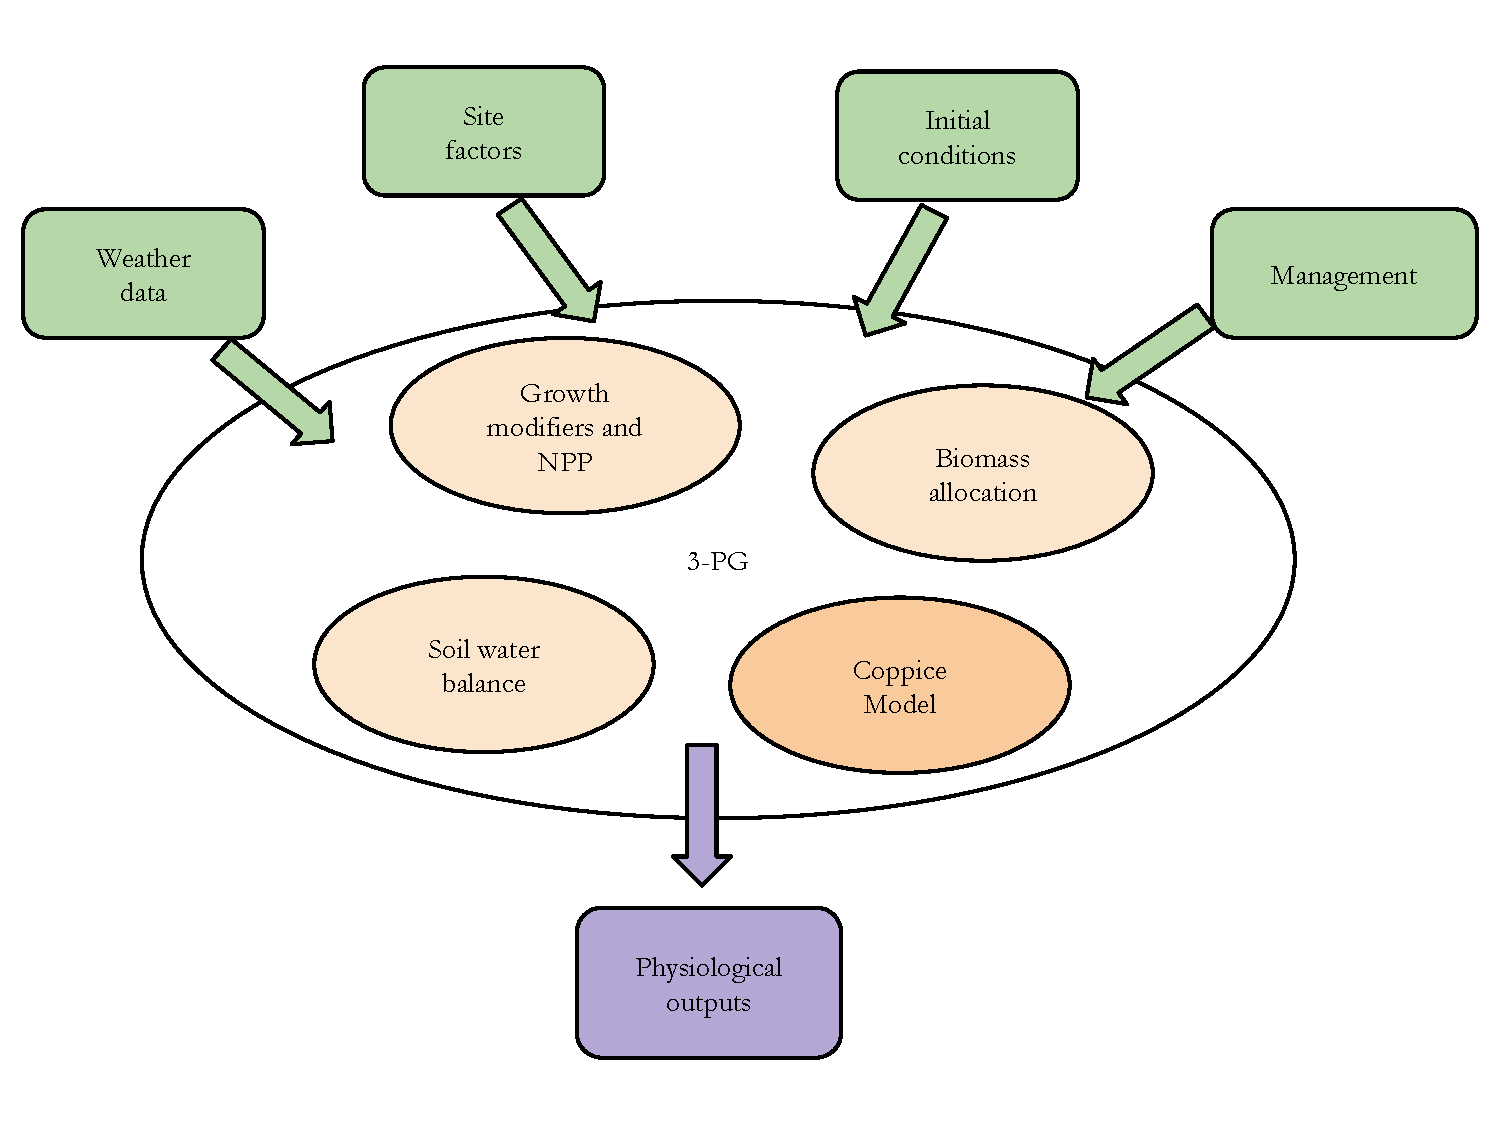
\includegraphics[width=\linewidth]{model_overview}
\caption{ \textbf{\ac{3pg} Overview.}}
\label{fig:growth-model}
\end{figure}

The \ac{3pg} model takes as inputs weather data, site factors, initial
conditions, management practices, and species information.  The model
typically runs at a monthly timestep. At each step the physiological
parameters are calculated and carried forward to the next month. Input
weather parameters are specified at the same monthly timestep, and
additional management parameters, such as irrigation scheduling, and
when the poplar is coppiced are also be included.

The physiological components of the \ac{3pg} model comprises of
sub-modules for estimating growth modifiers, \ac{NPP}, biomass
allocation, and soil water balance.  We have added an additional
sub-module to provide additional regrowth from an existing root mass,
primarily after a coppicing event.  In general, the \ac{3pg} model
works by predicting expected productivity based on the soil, the
current weather, and their interaction with the species under
consideration.  At each time step, a level of productivity is
calculated, This is basically potential maximum value, based on the
weather conditions, scaled with a number of multiplicative limiters
based on the plants response to temperature, water availability,
fertility, and other species dependent processes.

\subsubsection*{Poplar Hybrids parameterized for \ac{3pg}}

There have been a few studies specifically for modeling poplar using the
\ac{3pg} model~\cite{Amichev2010,Headlee2012}.  Headlee~\cite{Headlee2012} in
particular, developed a set of \pop parameters from a set of both laboratory and
field studies.  These parameters, with a few modifications, were used as the
control set to parameterize the growth of a representative hybrid poplar.  As
will be discussed below, when compared to field trials it can be seen that
different \pop clones can vary considerably in their growth patterns.  These
changes can be modeled with appropriate changes to the \ac{3pg} input
parameters.  Tables~\ref{tab:3pg-tree-productivity},
\ref{tab:3pg-tree-modifiers} and \ref{tab:3pg-tree-allocate} summarize the
control parameters used for the generic \pop model in this study.

\begin{table}[!ht]
\caption{\textbf{\ac{3pg} Model Productivity Parameters}}
\begin{tabularx}{\linewidth}{|c|X|c|}
  \hline
  Parameter & \centering{Source} & Value\\
  \hline
  $y$ & Assimilation use efficiency.  Used in calculation of the \NPP. & 0.47\\
  \hline  kG (kg Pa-1) & Determines the response of the canopy conductance to the vapor pressure deficit. & 0.5\\
  alpha (kg mol-1) & Canopy quantum efficiency. & 0.06\\
  \BLcond~(m-1) & Canopy boundary layer conductance. Used in the calcuation of transpiration & 0.2\\
  \hline
  $k$  & Radiation Extinction Coefficient & 0.5\\
  \SLA~(m2 kg-1) & Specific Leaf Area.  Defined as a function of the tree age.  Used in the calculation of LAI. &\\
  $f0_{\SLA}$ & \SLA~at initial time & 10.8\\
  $f1_{\SLA}$ & \SLA~at infinite timestep & 10.8\\
  $tm_{\SLA}$~(y) & Time in years where value is the average of $f0$ and $f1$ & 1\\
  $n$  & $n>=1$; Parameter specifing the rate of change around $tm$.  $n=1$ is approximately a linear change, as n increases, change becomes more localized around $tm$. & 2\\
  \hline
  % fullCanAge~(y) & Year where tree reaches full Canopy Cover. Used along with \LAI~in the productivity calculation & 1.5  \\
  % \hline
  % $Cond$~(m s-1) &  Canopy Conductance.  Along with a Physiological modifer, specifies the canopy conductance.  Used in calculation of transpiration & \\
  % $mn_{Cond}$ & Minimum value, when $lai=0$ & 0.0001\\
  % $mx_{Cond}$ & Maximum value & 0.02\\
  % $lai_{Cond}$~(m2 m-2) & \LAI where parameter reaches a maximum value. & 3.33\\
  % \hline
  % $Intcptn$ & Rainfall interception fraction. & \\
  % $mn_{Intcptn}$ & Minimum value, when $\LAI=0$ & 0\\
  % $mx_{Intcptn}$ & Maximum value & 0.15\\
  % $lai_{Intcptn}$~(m2 m-2) & \LAI~where parameter reaches a maximum value. & 5\\
  % \hline
\end{tabularx}


\begin{flushleft}Parameters primarily concerned with the overall productivity and transpiration of the plant.
\end{flushleft}
\label{tab:3pg-tree-productivity}
 \end{table}

\begin{table}[!ht]
\caption{\textbf{\ac{3pg} Growth Modifier Parameters}}
\begin{tabularx}{\linewidth}{|c|X|c|}
  \hline
  Parameter & \centering{Source} & Value\\
  \hline
  $y$ & Assimilation use efficiency.  Used in calculation of the \NPP. & 0.47\\
  \hline  kG (kg Pa-1) & Determines the response of the canopy conductance to the vapor pressure deficit. & 0.5\\
  alpha (kg mol-1) & Canopy quantum efficiency. & 0.06\\
  \BLcond~(m-1) & Canopy boundary layer conductance. Used in the calcuation of transpiration & 0.2\\
  \hline
  $k$  & Radiation Extinction Coefficient & 0.5\\
  \SLA~(m2 kg-1) & Specific Leaf Area.  Defined as a function of the tree age.  Used in the calculation of LAI. &\\
  $f0_{\SLA}$ & \SLA~at initial time & 10.8\\
  $f1_{\SLA}$ & \SLA~at infinite timestep & 10.8\\
  $tm_{\SLA}$~(y) & Time in years where value is the average of $f0$ and $f1$ & 1\\
  $n$  & $n>=1$; Parameter specifing the rate of change around $tm$.  $n=1$ is approximately a linear change, as n increases, change becomes more localized around $tm$. & 2\\
  \hline
  % fullCanAge~(y) & Year where tree reaches full Canopy Cover. Used along with \LAI~in the productivity calculation & 1.5  \\
  % \hline
  % $Cond$~(m s-1) &  Canopy Conductance.  Along with a Physiological modifer, specifies the canopy conductance.  Used in calculation of transpiration & \\
  % $mn_{Cond}$ & Minimum value, when $lai=0$ & 0.0001\\
  % $mx_{Cond}$ & Maximum value & 0.02\\
  % $lai_{Cond}$~(m2 m-2) & \LAI where parameter reaches a maximum value. & 3.33\\
  % \hline
  % $Intcptn$ & Rainfall interception fraction. & \\
  % $mn_{Intcptn}$ & Minimum value, when $\LAI=0$ & 0\\
  % $mx_{Intcptn}$ & Maximum value & 0.15\\
  % $lai_{Intcptn}$~(m2 m-2) & \LAI~where parameter reaches a maximum value. & 5\\
  % \hline
\end{tabularx}


\begin{flushleft}Parameters used in the determining species specific modifiers to the potential plant production.
\end{flushleft}
\label{tab:3pg-tree-modifiers}
 \end{table}

\begin{table}[!ht]
\caption{\textbf{\ac{3pg} Tree allocation Parameters}}
\begin{tabularx}{\linewidth}{|c|X|c|}
\hline
Parameter & Description & Value\\
\hline
 $pfs$ [frac]  & This defines the foliage to stem ($\frac{WF}{WS}$) fraction in allocating aboveground biomass of the tree. This is calculated with a pair of allometric power equations.  The first relates \acf{DOB} to total woody biomass, while the second relates \ac{DOB} to $pfs$.  The parameters of the relation between \ac{DOB} and woody biomass are inverted to determine the \ac{DOB} from the modeled woody fraction.&\\
 $stemCnt$ & Average number of stems per stump &2.8\\
 $stemC$ [$\reciprocal\centi\meter$] & Constant in relation of \ac{DOB} to woody biomass & 0.18\\
 $stemP$ & Power in relation of \ac{DOB} to woody biomass. & 2.4\\
 $pfsMx$ & Maximum possible pfs value allowed & 2\\
 $pfsP$ & Power in relation of \ac{DOB} to pfs & -1.161976\\
 $pfsC$ [$\reciprocal\centi\meter$] & Constant in relation of \ac{DOB} to $pfs$. & 1.92\\
 \hline
$pR$ [frac] & Along with a physiological parameter, specifies the amount of new growth allocated to the root system. &\\
 $mn_{pR}$ & Minimum allocation to the root, when the physiological parameter is 1. & 0.25\\
 $mx_{pR}$ & Maximum allocation to the root. & 0.34\\
 $m0_{pR}$ & Dependence on \ac{fR}. $m0=0$ indicates full dependence on fertility, $m0=1$ indicates a constant allocation, independent of fertility & 0\\
 $turnover$ & Specifies the monthly root turnover rate. & 0.005\\
% $turnover$ [$\reciprocal\unit[30.4]{\day}$] & Specifies the monthly root turnover rate. & 0.005\\
 \hline
 \ac{lf} [frac] & Specifies the fractional monthly loss of foliage. This is a time dependent parameter.&\\
 $f0_{\acs{lf}}$ & Value at initial timestep & 0.0015\\
 $f1_{\acs{lf}}$ & Value at infinite timestep & 0.03\\
 $tm_{\acs{lf}}$ [yr] & Time in years where value is the average of $f0$ and $f1$ & 2\\
 $n_{\acs{lf}}$  & $n>=1$; Specifies the rate of change around $tm$.  $n=1$ is approximately a linear change, as $n$ increases, change becomes more localized around $tm$. & 2.5\\
\hline
\end{tabularx}

\begin{flushleft}Parameters primarily used for predicting the allocation of growth among the components of the tree.
\end{flushleft}
\label{tab:3pg-tree-allocate}
 \end{table}

\subsection*{Coppicing Model}
\label{sec:coppicing-model}

The \ac{3pg} model allocates the monthly productivity from
transpiration of the trees into the creation of new roots, stems and
foliage.  In the standard \ac{3pg} model, the amount allocated to
roots is basically a constant allocation, potentially with a modifier
due to the plants fertility stress. The amount allocated to the
foliage and stems is dependent on the age and size of the trees.  In a
\ac{SRWC} however, coppicing the trees during harvesting introduces a
situation where the stem and foliage are removed, but the root ball
remains.  Because the original model derives it's production from
transpiration, the \ac{3pg} model has no mechanism to increase to
start re-growth from this situation.  In addition the model does not
moderate the allocations based on the abrupt changes in the composition
of the plant.

\begin{figure}[!ht]
\begin{subfigure}[b]{.1125\linewidth}
\centering
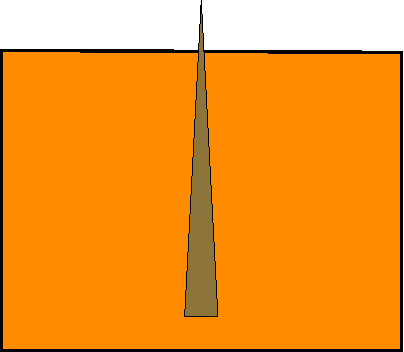
\includegraphics[width=1.0\linewidth]{img/tree_pics_1}
\caption{}  %\caption{planting}
\label{fig:grow_1}
\end{subfigure}
\begin{subfigure}[b]{.1125\linewidth}
\centering
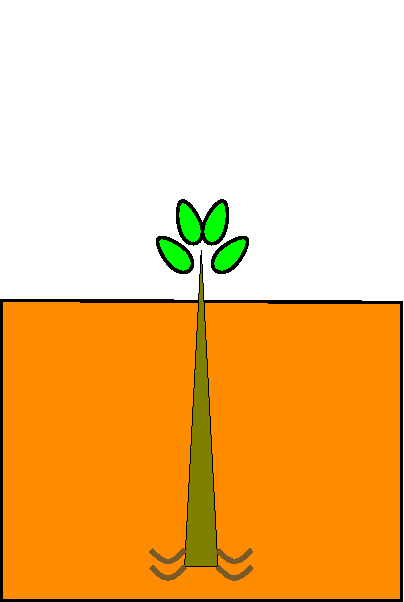
\includegraphics[width=1.0\linewidth]{img/tree_pics_2}
\caption{}  %\caption{sprout}
\label{fig:grow_2}
\end{subfigure}
\begin{subfigure}[b]{.1125\linewidth}
\centering
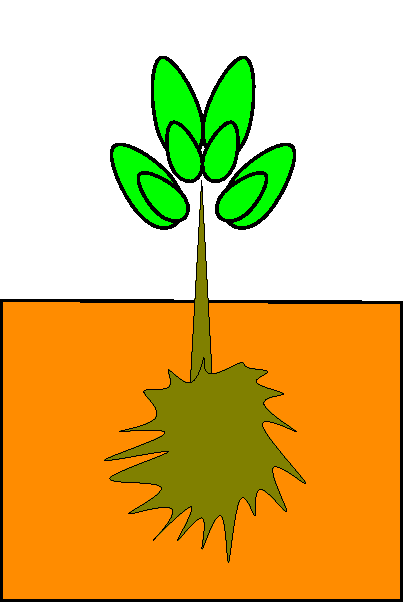
\includegraphics[width=1.0\linewidth]{img/tree_pics_3}
\caption{}  %\caption{growth}
\label{fig:grow_3}
\end{subfigure}
\begin{subfigure}[b]{.1125\linewidth}
\centering
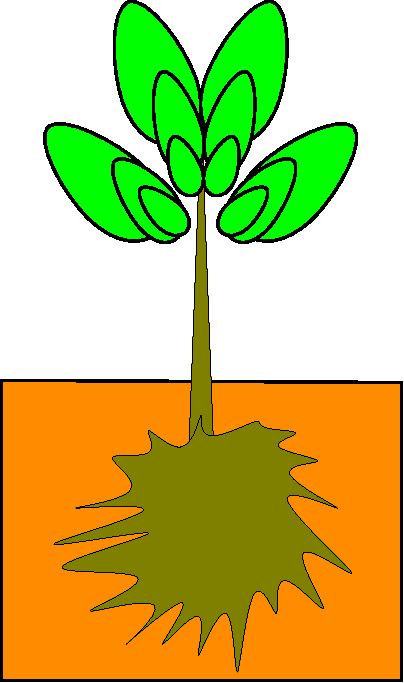
\includegraphics[width=1.0\linewidth]{img/tree_pics_4}
\caption{}  %\caption{maturity}
\label{fig:grow_4}
\end{subfigure}
\begin{subfigure}[b]{.1125\linewidth}
\centering
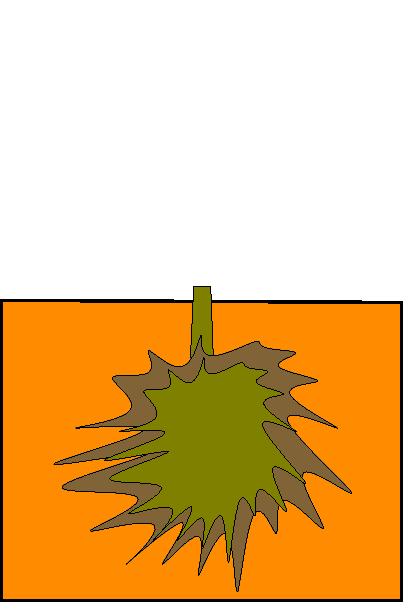
\includegraphics[width=1.0\linewidth]{img/tree_pics_5}
\caption{}  %\caption{coppiced}
\label{fig:grow_5}
\end{subfigure}
\begin{subfigure}[b]{.1125\linewidth}
\centering
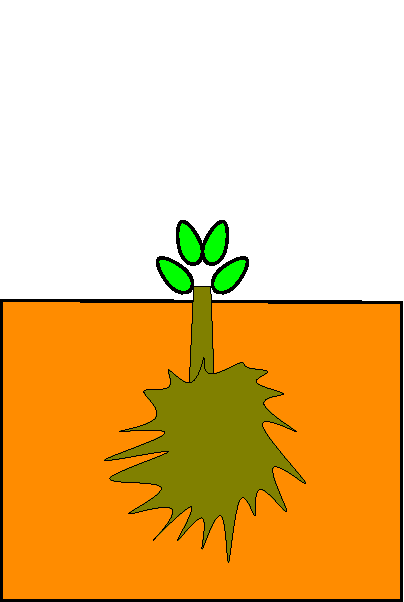
\includegraphics[width=1.0\linewidth]{img/tree_pics_6}
\caption{}  %\caption{resprouting}
\label{fig:grow_6}
\end{subfigure}
\begin{subfigure}[b]{.1125\linewidth}
\centering
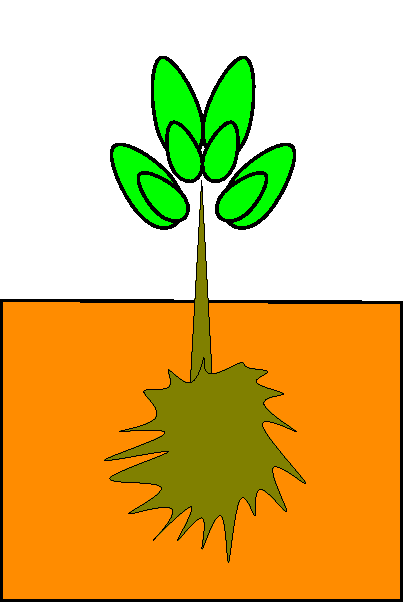
\includegraphics[width=1.0\linewidth]{img/tree_pics_7}
\caption{}  %\caption{regrowth}
\label{fig:grow_7}
\end{subfigure}
\begin{subfigure}[b]{.1125\linewidth}
\centering
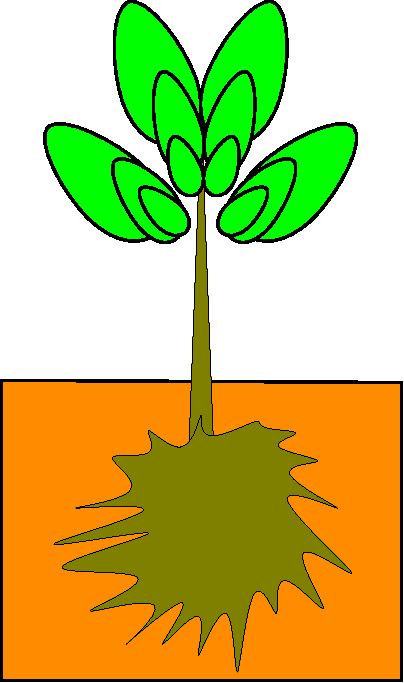
\includegraphics[width=1.0\linewidth]{img/tree_pics_4}
\caption{}  %\caption{next harvest}
\label{fig:grow_8}
\end{subfigure}
\caption{ \textbf{Poplar \ac{SRWC} growth.} The growth stages for poplar
  grown as an \ac{SRWC} with one coppicing cycle shown. }
\label{fig:grow}
\end{figure}

Figure~\ref{fig:grow} shows the typical growth of a poplar planted as
a \ac{SRWC}.  Poplars are generally propagated via cuttings of bare
poplar stem, mostly under the soil,~(Figure~\ref{fig:grow_1}).  The
cutting provides energy for the establishment of the seedling via buds
above and below the surface~(Figure~\ref{fig:grow_2}). As the poplar
matures, it is the productivity provided by the plant's transpiration
that provides for growth.  This includes the establishment of the root
ball~(Figure~\ref{fig:grow_3}).  By the time the poplar is ready for
coppicing~(Figure~\ref{fig:grow_4}), the plants are well established.

After coppicing, there is a surfeit of root mass, and no foliage to
provide photosynthetic based productivity to the
tree~(Figure~\ref{fig:grow_5}).  However, a portion of the root mass
is available as a production source for the tree.  Sometime later, the
tree resprouts with the root ball providing initial energy for the
reestablishment of seedlings~(Figure~\ref{fig:grow_6}). In most
species, resprouting will occur among multiple stems from the same
root.  Re-sprouting leads through the maturation of the poplar, ready for
the next harvest~(Figures~\ref{fig:grow_7} and~\ref{fig:grow_8}).
Modeling the growth of the \ac{SRWC} then becomes, in part, a task of
determining the size and timing of the regrowth from the existing root
mass.

We have developed a simple root interaction system added to the
\ac{3pg} model to model the behavior both of the post-coppiced
situation as well as the initial planting of the cutting. At any given
timestep the model augments the productivity from the plant's
transpiration with an additional production from utilization of
reserves with in the root mass.  Under normal conditions, this
augmentation is zero, however, with the initial planting of the
cutting, or after a coppicing event, this augmentation is used to add
foliage to the tree and restart transpiration based production.

The parameters of the model are shown in figure~\ref{fig:coppice}.
Three species specific parameters control the coppicing model.
Combined with the input weather, and some parameters in the \ac{3pg}
model, these control the extent and the timing of the regrowth from
the coppiced plant.

\begin{figure}[!ht]
  \centering
\begin{subfigure}[b]{.2\linewidth}
  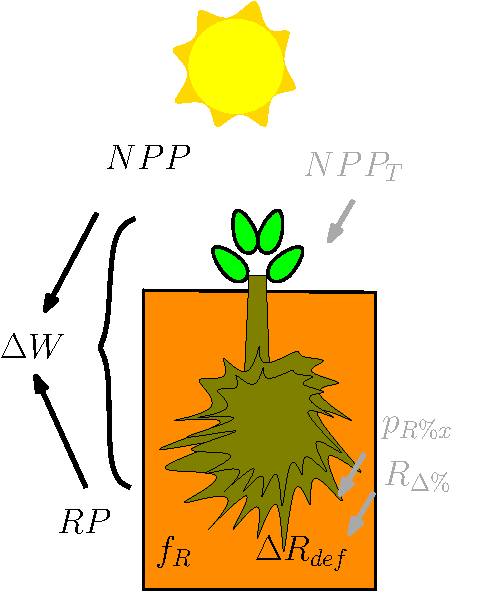
\includegraphics[width=1.0\linewidth]{img/tree_pics_10}
%  \caption{Parameters}
%  \label{fig:coppice-img}
\end{subfigure}
\quad
\begin{subtable}[b]{.75\linewidth}
\begin{align}
\acs{dW}=\acs{NPP}+\acs{RP} \\
\acs{RP} = \begin{cases} 0 & \acs{NPPdef} <=0 \\
\acs{fR} ~ min (\acs{dRres} ,\acs{NPPdef}) & \acs{NPPdef} > 0  
\end{cases} \\
\acs{NPPdef} = \acs{NPPt}-\acs{NPP} \\
\acs{dRres} = \acs{WR}(\acs{WR}/\acs{W} - \acs{pRx})\acs{Rdp}
\end{align}
%\caption{Model Definition}
\end{subtable}
\caption{\textbf{Coppice Model Overview}}
\label{fig:coppice}
\end{figure}

The model is designed to integrate easily into that existing \ac{3pg}
equations, with only limited modifications.  To that end, at each monthly
timestep, the model allocates it's productivity as before.  The only
difference being that \acf{dW} is now the sum of the \acf{NPP} and an
additional \acf{RP}.  The contribution from \ac{RP} however, is
dependent on the weather, the state of the plant, and some parameters
defining the root mass characteristics. 

The contribution \ac{RP} is affected by the potential of a plant to
grow under the current weather conditions, as defined by the potential
productivity of the plant.  \ac{NPPt} defines a target productivity
within a given timestep.  This target can in turn be defined with
\acs{LAIt}, a target \ac{LAI} which may or may not be realized by
tree's current distribution .  The \acs{LAIt} parameter can be thought
of as defining a minimum operational \acs{NPP} which the plant
attempting to reach.  \acs{LAIt} can vary from 0 and greater.  A value
of 0 indicates no root contribution, where higher values indicate
contribution from the roots even as the plant is producing higher
values for \acs{NPP} from it's foliage.

This affects the timing of the root contribution, because the
\ac{NPPt} is affected by the current weather conditions.  If those
conditions are not conducive to plant transpiration, then \ac{NPPt} is
low, and resources are not allocated for growth.  \ac{NPPdef} is then
defined as the difference between the \ac{NPPt} and
\ac{NPP}. \ac{NPPdef} defines a maximum contribution from the roots to
the overall plant growth.  The actual contribution is also limited by
the amount of energy available in the root mass at any given timestep.

As described above, \ac{3pg} model defines a root allocation
parameter, \acs{pRx}, which defines the root size with respect to the
entire plant size.  After coppicing, the root mass is larger then
\acs{pRx}.  Some amount of that extra root mass,\acs{dRres} will be
made available for production.  The parameter, \ac{Rdp}, (ranging from
0 to 1), defines what fraction this surplus root mass can contribute
to \ac{RP} in a given timestep.  A value of 0 indicates no root
contribution for regrowth, higher values indicate more potential
growth available to the plant at each timestep.

Finally, the parameter \acf{fR}, ranging from 0 to 1, determines the
efficiency of the contribution, in effect, determining the fraction of
new mass of growth, to loss of root mass.  \acs{fR} is multiplied with
the available root mass to determine \ac{RP}.

In poplar plantations, initially planted with cuttings, original
growth is modeled the same way.  A different set of parameters for
\ac{LAIt},\ac{Rdp}, and \acs{fR} can be used for the cutting and the
post-coppiced trees.  Because poplars are typically propagated from
cuttings, some of the parameters of the tree vary between the initial
planting and a coppicing event.  Because of this, we have altered our
model to allow for a different set of tree parameters to be associated
with the original cutting, and the post coppiced tree.  These
differences have been limited to changes in the root parameters.

Figures~\ref{fig:date},~\ref{fig:rdp} and~\ref{fig:lai} illustrate the
effect of these parameters on the expected plant growth.  For these
examples, the climatic parameters shown in
Figure~\ref{fig:weather} were used.  The plants were also never
limited by water availability.

\begin{figure}
  \centering
%  \begin{tikzpicture}
  \begin{axis}[
    no markers,
    width=\linewidth,
    height=2in,
    date coordinates in=x,
    xticklabel={\month},
    ylabel style={align=center}, ylabel=Rad {$[MJ/day]$}; Temp {$[C]$}\\ Daylight {$[hr]$},
    stack plots=false,
    bar width=2pt,
    legend entries={$T_n$,$T_x$,$R$,$Hrs$},
    legend style={at={(0.4,1.03)},anchor=south},
    legend columns=4,
    %legend to name = temp
    % legend style={
    % at={(0.5,-0.3)},anchor=north,legend columns=-1}
    ]
    \addplot+[color=yellow] table [x=date, y=tmin, col sep=comma] {coppice/weather.csv};
    \addplot+[color=red ] table [x=date, y=tmax, col sep=comma] {coppice/weather.csv};
    \addplot+[ybar, color=blue, fill=blue] table [x=date, y=rad, col sep=comma] {coppice/weather.csv};
    \addplot+[ybar, color=green, fill=green] table [x=date, y=daylight, col sep=comma] {coppice/weather.csv};
    
  \end{axis}
  \begin{axis}[
     no markers,
     width=\linewidth,
     height=2in,
     date coordinates in=x,
  %   ylabel=PPT [mm],
     axis y line=right,
     axis x line=none,
  %   % ylabel style={yshift=10pt},
     legend entries={$PPT$},
     legend style={
        at={(.7,1.03)},
        anchor=south},
     %legend to name = ppt,
     ylabel style={align=center}, ylabel=Precip {$[mm]$},
     ]
    \addplot+[color=black] table [x=date, y=ppt, col sep=comma] {coppice/weather.csv};
   \end{axis}
\end{tikzpicture}
%\ref{temp}

  \caption{Illustrative weather data, replicating conditions similar
    to those found in Corvallis, OR}
  \label{fig:weather}
\end{figure}

A plant parameterized with $\ac{Rdp}=1$, $\acs{fR}=1$ and
$\acs{LAIt}=100$ will reallocate the maximum resources back into plant
growth as fast as possible.  This is an illustrative example to show
the affect of the season on the modeled regrowth.
Figure~\ref{fig:date} shows the response of this plant for various
coppicing dates.

\begin{figure}
  \centering
  \pgfplotsset{
      no markers,
      width=\linewidth,
      height=0.25\linewidth,
      every axis plot/.append style={line width=1pt},
      date coordinates in=x,
      xmin={2016-02-15},
      xmax={2019-10-15},
      xtick={2016-06-15,2016-09-15,2016-12-15,
      2017-03-15,2017-06-15,2017-09-15,2017-12-15,
      2018-03-15,2018-06-15,2018-09-15,2018-12-15,
      2019-03-15,2019-06-15,2019-09-15},
      x tick label style={rotate=45, anchor=east},
      xticklabels={Y2-06,Y2-09,Y2-12,
      Y3-03,Y3-06,Y3-09,Y3-12,
      Y4-03,Y4-06,Y4-09,Y4-12,
      Y5-03,Y5-06,Y5-09},
      ymin=0,ymax=60,
      ytick={20,40},
      yticklabels={20,40},
}
  \begin{tikzpicture}
    \begin{axis}[
      name=feb,
      legend entries={Stem,Root,Foilage},
      legend style={
        at={(0.5,1)},anchor=south,legend columns=-1,yshift=1pt},
      xticklabels=\empty,
      ]
      \node[right] at (axis cs:{2016-02-15},50) {Y3-02};
      \addplot+[color=brown] table [x=date, y=m02f1, col sep=comma] {coppice/hart12coppice-coppice-ws.csv};
      \addplot+[color=red] table [x=date, y=m02f1, col sep=comma] {coppice/hart12coppice-coppice-wr.csv};
      \addplot+[color=green] table [x=date, y=m02f1, col sep=comma] {coppice/hart12coppice-coppice-wf.csv};
    \end{axis}
    \begin{axis}[
      name=may,
      at={(feb.below south west)},yshift=5pt,
      anchor=north west,
      xticklabels=\empty,
      ]
      \node[right] at (axis cs:{2016-02-15},50) {Y3-05};
      \addplot+[color=brown] table [x=date, y=m05f1, col sep=comma] {coppice/hart12coppice-coppice-ws.csv};
      \addplot+[color=red] table [x=date, y=m05f1, col sep=comma] {coppice/hart12coppice-coppice-wr.csv};
      \addplot+[color=green] table [x=date, y=m05f1, col sep=comma] {coppice/hart12coppice-coppice-wf.csv};
    \end{axis}
    \begin{axis}[
      name=aug,
      at={(may.below south west)},yshift=5pt,
      anchor=north west,
      xticklabels=\empty,
      ]
      \node[right] at (axis cs:{2016-02-15},50) {Y3-08};
      \addplot+[color=brown] table [x=date, y=m08f1, col sep=comma] {coppice/hart12coppice-coppice-ws.csv};
      \addplot+[color=red] table [x=date, y=m08f1, col sep=comma] {coppice/hart12coppice-coppice-wr.csv};
      \addplot+[color=green] table [x=date, y=m08f1, col sep=comma] {coppice/hart12coppice-coppice-wf.csv};
    \end{axis}
    \begin{axis}[
      name=nov,
      at={(aug.below south west)},yshift=5pt,
      anchor=north west,
      height=0.2916\linewidth,
      ymin=0,ymax=70,
      ytick={20,40,60},
      yticklabels={20,40,60},
      ]
      \node[right] at (axis cs:{2016-02-15},50) {Y3-11};
      \addplot+[color=brown] table [x=date, y=m11f1, col sep=comma] {coppice/hart12coppice-coppice-ws.csv};
      \addplot+[color=red] table [x=date, y=m11f1, col sep=comma] {coppice/hart12coppice-coppice-wr.csv};
      \addplot+[color=green] table [x=date, y=m11f1, col sep=comma] {coppice/hart12coppice-coppice-wf.csv};
    \end{axis}
  \end{tikzpicture}

  \caption{Coppice regrowth model results for various coppicing dates.
    Y-axis is the dry mass of each component of the plantation, in
    terms of $\frac{T}{ha}$.}
  \label{fig:date}
\end{figure}

These figures show the predicted amounts of biomass partitioned among
stem, root and foliage.  Coppicing is modeled in the third year, in
February, May, August, or November.  The results predicted by the each
coppicing event are shown.  During periods with high potential
productivity, roots contribute more quickly to the regrowth of the
stem and foliage, matching the higher potential \ac{NPP}.  Late season
harvests defer their growth until the following spring conditions, and
at a slower rate to match the lower potential productivity at those
times.  The total production of the plantation, is affected by the
timing of the coppicing.  Even with the root contribution, this is due
to a lost opportunity for production during the growing season.

The model predictions show the total foliage and root biomass
converging to similar values for all of the coppicing dates.

Figure~\ref{fig:rdp} shows the model variation from various values for
\acf{Rdp}.  In these graphs, the foliage, stem, and root mass are
compared for two separate coppicing dates for the third year growth in
August and November.  The value for \ac{Rdp} ranges from 0.001 to 1.

\begin{figure}
  \centering
  \pgfplotsset{
      no markers,
      width=0.5\linewidth,
      height=0.25\linewidth,
      every axis plot/.append style={line width=1pt},
      date coordinates in=x,
      xmin={2017-03-15},
      xmax={2019-10-15},
      xtick={
      2017-06-15,2017-09-15,2017-12-15,
      2018-03-15,2018-06-15,2018-09-15,2018-12-15,
      2019-03-15,2019-06-15,2019-09-15},
      xticklabels=\empty,
}
  \begin{tikzpicture}
    \begin{axis}[
      name=ws08,
      ymin=0,ymax=80,
      ytick={20,40,60},
      yticklabels={20,40,60},
      ylabel=Stem~$\frac{T}{ha}$,
      legend entries={$\Rdp=0.001$,$\Rdp=0.01$,$\Rdp=0.1$,$\Rdp=0.5$,$\Rdp=1$},
      legend style={
        at={(1.0,1.0)},anchor=south,legend columns=-1,yshift=2pt}
      ]
      \node[right] at (axis cs:{2018-02-15},50) {Aug};
      \addplot+[color=red] table [x=date, y=m08f0.001, col sep=comma] {coppice/hart12coppice-coppice-ws.csv};
      \addplot+[color=orange] table [x=date, y=m08f0.01, col sep=comma] {coppice/hart12coppice-coppice-ws.csv};
      \addplot+[color=yellow] table [x=date, y=m08f0.1, col sep=comma] {coppice/hart12coppice-coppice-ws.csv};
      \addplot+[color=green] table [x=date, y=m08f0.5, col sep=comma] {coppice/hart12coppice-coppice-ws.csv};
      \addplot+[color=blue] table [x=date, y=m08f1, col sep=comma] {coppice/hart12coppice-coppice-ws.csv};
    \end{axis}
    \begin{axis}[
      name=ws11,
      at={(ws08.east)},xshift=2pt,
      anchor=west,
      ymin=0,ymax=80,
      ytick={20,40,60},
      yticklabels=\empty
      ]
      \node at (axis cs:{2018-02-15},50) {Nov};
      \addplot+[color=red] table [x=date, y=m11f0.001, col sep=comma] {coppice/hart12coppice-coppice-ws.csv};
      \addplot+[color=orange] table [x=date, y=m11f0.01, col sep=comma] {coppice/hart12coppice-coppice-ws.csv};
      \addplot+[color=yellow] table [x=date, y=m11f0.1, col sep=comma] {coppice/hart12coppice-coppice-ws.csv};
      \addplot+[color=green] table [x=date, y=m11f0.5, col sep=comma] {coppice/hart12coppice-coppice-ws.csv};
      \addplot+[color=blue] table [x=date, y=m11f1, col sep=comma] {coppice/hart12coppice-coppice-ws.csv};
    \end{axis}

    \begin{axis}[
      name=wf08,
      ylabel=Foilage,
      at={(ws08.below south west)},yshift=5pt,
      anchor=north west,
      ymin=0,ymax=30,
      ytick={10,20},
      yticklabels={10,20},
      ]
%      \node[right] at (axis cs:{2016-02-15},50) {Aug};
      \addplot+[color=red] table [x=date, y=m08f0.001, col sep=comma] {coppice/hart12coppice-coppice-wf.csv};
      \addplot+[color=orange] table [x=date, y=m08f0.01, col sep=comma] {coppice/hart12coppice-coppice-wf.csv};
      \addplot+[color=yellow] table [x=date, y=m08f0.1, col sep=comma] {coppice/hart12coppice-coppice-wf.csv};
      \addplot+[color=green] table [x=date, y=m08f0.5, col sep=comma] {coppice/hart12coppice-coppice-wf.csv};
      \addplot+[color=blue] table [x=date, y=m08f1, col sep=comma] {coppice/hart12coppice-coppice-wf.csv};
    \end{axis}

    \begin{axis}[
      name=wf11,
      at={(wf08.east)},xshift=2pt,
      anchor=west,
      ymin=0,ymax=30,
      ytick={10,20},
      yticklabels=\empty
      ]
%      \node[right] at (axis cs:{2016-02-15},50) {Nov};
      \addplot+[color=red] table [x=date, y=m11f0.001, col sep=comma] {coppice/hart12coppice-coppice-wf.csv};
      \addplot+[color=orange] table [x=date, y=m11f0.01, col sep=comma] {coppice/hart12coppice-coppice-wf.csv};
      \addplot+[color=yellow] table [x=date, y=m11f0.1, col sep=comma] {coppice/hart12coppice-coppice-wf.csv};
      \addplot+[color=green] table [x=date, y=m11f0.5, col sep=comma] {coppice/hart12coppice-coppice-wf.csv};
      \addplot+[color=blue] table [x=date, y=m11f1, col sep=comma] {coppice/hart12coppice-coppice-wf.csv};
    \end{axis}

    \begin{axis}[
      name=wr08,
      at={(wf08.below south west)},yshift=5pt,
      anchor=north west,
      x tick label style={rotate=45, anchor=east},
      xticklabels={
      Y3-06,Y3-09,Y3-12,
      Y4-03,Y4-06,Y4-09,Y4-12,
      Y5-03,Y5-06,Y5-09},
      ymin=5,ymax=30,
      ytick={10,20},
      yticklabels={10,20},
      ylabel=Root,
      ]
%      \node[right] at (axis cs:{2016-02-15},30) {Aug};
      \addplot+[color=red] table [x=date, y=m08f0.001, col sep=comma] {coppice/hart12coppice-coppice-wr.csv};
      \addplot+[color=orange] table [x=date, y=m08f0.01, col sep=comma] {coppice/hart12coppice-coppice-wr.csv};
      \addplot+[color=yellow] table [x=date, y=m08f0.1, col sep=comma] {coppice/hart12coppice-coppice-wr.csv};
      \addplot+[color=green] table [x=date, y=m08f0.5, col sep=comma] {coppice/hart12coppice-coppice-wr.csv};
      \addplot+[color=blue] table [x=date, y=m08f1, col sep=comma] {coppice/hart12coppice-coppice-wr.csv};
    \end{axis}

    \begin{axis}[
      name=wr11,
      at={(wr08.east)},xshift=2pt,
      anchor=west,
      yticklabels=\empty,
      x tick label style={rotate=45, anchor=east},
      xticklabels={
      Y3-06,Y3-09,Y3-12,
      Y4-03,Y4-06,Y4-09,Y4-12,
      Y5-03,Y5-06,Y5-09},
      ymin=5,ymax=30,
      ytick={10,20},
      yticklabels=\empty,
      ]
%      \node[right] at (axis cs:{2016-02-15},30) {Nov};
      \addplot+[color=red] table [x=date, y=m11f0.001, col sep=comma] {coppice/hart12coppice-coppice-wr.csv};
      \addplot+[color=orange] table [x=date, y=m11f0.01, col sep=comma] {coppice/hart12coppice-coppice-wr.csv};
      \addplot+[color=yellow] table [x=date, y=m11f0.1, col sep=comma] {coppice/hart12coppice-coppice-wr.csv};
      \addplot+[color=green] table [x=date, y=m11f0.5, col sep=comma] {coppice/hart12coppice-coppice-wr.csv};
      \addplot+[color=blue] table [x=date, y=m11f1, col sep=comma] {coppice/hart12coppice-coppice-wr.csv};
    \end{axis}

  \end{tikzpicture}

  \caption{Coppice regrowth model results for various levels of \acf{Rdp}.
    Y-axis is the dry mass of each component of the plantation, in
    terms of $\frac{T}{ha}$. $\ac{Rdp}=100$ and $\ac{fR}=1$.}
  \label{fig:rdp}
\end{figure}

The figure shows a long term decrease in plant growth for very low
values of \ac{Rdp}, but values of \ac{Rdp} over about .1, the foliage
and stem growth are very similar after the first 6 months of growth.
This is because while the root's contribution to the plants
productivity is smaller for lower values if \ac{Rdp} it does continue
to contribute at each timestep while the root mass overly large. The
root mass itself shows large differences over a longer period for
these variations in \ac{Rdp}.  

The comparisons are closer for November, as the potential
productivities are smaller in the early months, and the lower values
of \ac{Rdp} can still provide enough production to match the
environmental conditions.

For modeling actual plants, values of \ac{Rdp} approaching 1 are
unlikely, as that \ac{Rdp} indicates mass that can be easily converted
to energy for the plants, primarily starches and sugars.  For poplar
in particular, roots' starch and sugar contents vary with the root
diameter, and range from low values to as much as 20\%.  A value of
$\ac{Rdp}=0.1$ is used for the comparisons to the field trials below. 

Figure~\ref{fig:lai} shows the change of the model with respect to the
change in the \ac{LAIt} value.  The figure shows the same coppicing
events as Figure~\ref{fig:rdp}, August and November events after 3
years of growth.  \ac{Rdp} is set to 10\%.  The figure shows very
little dependence on the \ac{LAIt} parameter as \ac{LAIt} is greater
than about 1.

\begin{figure}
  \centering
  \pgfplotsset{
      no markers,
      width=0.5\linewidth,
      height=0.25\linewidth,
      every axis plot/.append style={line width=1pt},
      date coordinates in=x,
      xmin={2017-03-15},
      xmax={2019-10-15},
      xtick={
      2017-06-15,2017-09-15,2017-12-15,
      2018-03-15,2018-06-15,2018-09-15,2018-12-15,
      2019-03-15,2019-06-15,2019-09-15},
      xticklabels=\empty,
}
  \begin{tikzpicture}
    \begin{axis}[
      name=ws08,
      ymin=0,ymax=80,
      ytick={20,40,60},
      yticklabels={20,40,60},
      ylabel=Stem~$\frac{T}{ha}$,
      legend entries={$\LAIt=0.1$,$\LAIt=1$,$\LAIt=10$},
      legend style={
        at={(1.0,1.0)},anchor=south,legend columns=-1,yshift=2pt}
      ]
      \node[right] at (axis cs:{2018-02-15},50) {Aug};
%      \addplot+[color=red] table [x=date, y=m08f0.1lai0, col sep=comma] {coppice/hart12coppice-lai-ws.csv};
      \addplot+[color=orange] table [x=date, y=m08f0.1lai0.1, col sep=comma] {coppice/hart12coppice-lai-ws.csv};
      \addplot+[color=yellow] table [x=date, y=m08f0.1lai1, col sep=comma] {coppice/hart12coppice-lai-ws.csv};
      \addplot+[color=green] table [x=date, y=m08f0.1lai10, col sep=comma] {coppice/hart12coppice-lai-ws.csv};
%      \addplot+[color=green] table [x=date, y=m08f1lai0.1, col sep=comma] {coppice/hart12coppice-lai-ws.csv};
%      \addplot+[color=blue] table [x=date, y=m08f1lai1, col sep=comma] {coppice/hart12coppice-lai-ws.csv};
    \end{axis}
    \begin{axis}[
      name=ws11,
      at={(ws08.east)},xshift=2pt,
      anchor=west,
      ymin=0,ymax=80,
      ytick={20,40,60},
      yticklabels=\empty
      ]
      \node at (axis cs:{2018-02-15},50) {Nov};
%      \addplot+[color=red] table [x=date, y=m11f0.1lai0, col sep=comma] {coppice/hart12coppice-lai-ws.csv};
      \addplot+[color=orange] table [x=date, y=m11f0.1lai0.1, col sep=comma] {coppice/hart12coppice-lai-ws.csv};
      \addplot+[color=yellow] table [x=date, y=m11f0.1lai1, col sep=comma] {coppice/hart12coppice-lai-ws.csv};
      \addplot+[color=green] table [x=date, y=m11f0.1lai10, col sep=comma] {coppice/hart12coppice-lai-ws.csv};
%      \addplot+[color=green] table [x=date, y=m11f1lai0.1, col sep=comma] {coppice/hart12coppice-lai-ws.csv};
%      \addplot+[color=blue] table [x=date, y=m11f1lai1, col sep=comma] {coppice/hart12coppice-lai-ws.csv};
    \end{axis}

    \begin{axis}[
      name=wf08,
      ylabel=Foilage,
      at={(ws08.below south west)},yshift=5pt,
      anchor=north west,
      ymin=0,ymax=30,
      ytick={10,20},
      yticklabels={10,20},
      ]
%      \node[right] at (axis cs:{2016-02-15},50) {Aug};
%      \addplot+[color=red] table [x=date, y=m08f0.1lai0, col sep=comma] {coppice/hart12coppice-lai-wf.csv};
      \addplot+[color=orange] table [x=date, y=m08f0.1lai0.1, col sep=comma] {coppice/hart12coppice-lai-wf.csv};
      \addplot+[color=yellow] table [x=date, y=m08f0.1lai1, col sep=comma] {coppice/hart12coppice-lai-wf.csv};
      \addplot+[color=green] table [x=date, y=m08f0.1lai10, col sep=comma] {coppice/hart12coppice-lai-wf.csv};
%      \addplot+[color=green] table [x=date, y=m08f1lai0.1, col sep=comma] {coppice/hart12coppice-lai-wf.csv};
%      \addplot+[color=blue] table [x=date, y=m08f1lai1, col sep=comma] {coppice/hart12coppice-lai-wf.csv};
    \end{axis}

    \begin{axis}[
      name=wf11,
      at={(wf08.east)},xshift=2pt,
      anchor=west,
      ymin=0,ymax=30,
      ytick={10,20},
      yticklabels=\empty
      ]
%      \node[right] at (axis cs:{2016-02-15},50) {Nov};
%      \addplot+[color=red] table [x=date, y=m11f0.1lai0, col sep=comma] {coppice/hart12coppice-lai-wf.csv};
      \addplot+[color=orange] table [x=date, y=m11f0.1lai0.1, col sep=comma] {coppice/hart12coppice-lai-wf.csv};
      \addplot+[color=yellow] table [x=date, y=m11f0.1lai1, col sep=comma] {coppice/hart12coppice-lai-wf.csv};
      \addplot+[color=green] table [x=date, y=m11f0.1lai10, col sep=comma] {coppice/hart12coppice-lai-wf.csv};
%      \addplot+[color=green] table [x=date, y=m11f1lai0.1, col sep=comma] {coppice/hart12coppice-lai-wf.csv};
%      \addplot+[color=blue] table [x=date, y=m11f1lai1, col sep=comma] {coppice/hart12coppice-lai-wf.csv};
    \end{axis}

    \begin{axis}[
      name=wr08,
      at={(wf08.below south west)},yshift=5pt,
      anchor=north west,
      x tick label style={rotate=45, anchor=east},
      xticklabels={
      Y3-06,Y3-09,Y3-12,
      Y4-03,Y4-06,Y4-09,Y4-12,
      Y5-03,Y5-06,Y5-09},
      ymin=5,ymax=30,
      ytick={10,20},
      yticklabels={10,20},
      ylabel=Root,
      ]
%      \node[right] at (axis cs:{2016-02-15},30) {Aug};
%      \addplot+[color=red] table [x=date, y=m08f0.1lai0, col sep=comma] {coppice/hart12coppice-lai-wr.csv};
      \addplot+[color=orange] table [x=date, y=m08f0.1lai0.1, col sep=comma] {coppice/hart12coppice-lai-wr.csv};
      \addplot+[color=yellow] table [x=date, y=m08f0.1lai1, col sep=comma] {coppice/hart12coppice-lai-wr.csv};
      \addplot+[color=green] table [x=date, y=m08f0.1lai10, col sep=comma] {coppice/hart12coppice-lai-wr.csv};
%      \addplot+[color=green] table [x=date, y=m08f1lai0.1, col sep=comma] {coppice/hart12coppice-lai-wr.csv};
%      \addplot+[color=blue] table [x=date, y=m08f1lai1, col sep=comma] {coppice/hart12coppice-lai-wr.csv};
    \end{axis}

    \begin{axis}[
      name=wr11,
      at={(wr08.east)},xshift=2pt,
      anchor=west,
      yticklabels=\empty,
      x tick label style={rotate=45, anchor=east},
      xticklabels={
      Y3-06,Y3-09,Y3-12,
      Y4-03,Y4-06,Y4-09,Y4-12,
      Y5-03,Y5-06,Y5-09},
      ymin=5,ymax=30,
      ytick={10,20},
      yticklabels=\empty,
      ]
%      \node[right] at (axis cs:{2016-02-15},30) {Nov};
%      \addplot+[color=red] table [x=date, y=m11f0.1lai0, col sep=comma] {coppice/hart12coppice-lai-wr.csv};
      \addplot+[color=orange] table [x=date, y=m11f0.1lai0.1, col sep=comma] {coppice/hart12coppice-lai-wr.csv};
      \addplot+[color=yellow] table [x=date, y=m11f0.1lai1, col sep=comma] {coppice/hart12coppice-lai-wr.csv};
      \addplot+[color=green] table [x=date, y=m11f0.1lai10, col sep=comma] {coppice/hart12coppice-lai-wr.csv};
%      \addplot+[color=green] table [x=date, y=m11f1lai0.1, col sep=comma] {coppice/hart12coppice-lai-wr.csv};
%      \addplot+[color=blue] table [x=date, y=m11f1lai1, col sep=comma] {coppice/hart12coppice-lai-wr.csv};
    \end{axis}

  \end{tikzpicture}

  \caption{Coppice regrowth model results for various levels of
    \acf{LAIt}.  $\ac{Rdp} = 0.1$ and $\ac{fR}=1$.  Y-axis is the dry
    mass of each component of the plantation, in terms of
    $\frac{T}{ha}$.}
  \label{fig:lai}
\end{figure}

\ac{LAI} is chosen as the primary target parameter for the \ac{3pg} as
it is a simple plant parameter controlling productivity.  It's primary
affect at a given timestep is that it affects the light gathering for
the tree.  That fraction is given in the \ac{3pg} model as $1-\exp{-k
  LAI}$.  For poplar we have defined $k=0.5$, and the productivity of
the tree starts to become dominated with this term for relatively low
values of \ac{LAI}.

Table~\ref{tab:3pg-tree-coppice} shows the parameters related to coppicing
chosen for the \ac{3pg} model.  They vary slightly between the planted cutting
and the subsequently coppiced trees.

\begin{table}[!ht]
\caption{\textbf{\ac{3pg} Coppicing Parameters}}
\begin{tabularx}{\linewidth}{|c|X|c|c|}
  \hline
  Parameter & Description & Cutting & Coppiced\\
\hline
pRx $[\unit{mo}\reciprocal]$ & The fractional amount of root biomass that exceeds the aboveground requirements that can be supplied in a given month. & 0.01 & 0.1\\
%\ac{pRx} $[\unit{mo}\reciprocal]$ & The fractional amount of root biomass that exceeds the aboveground requirements that can be supplied in a given month. & 0.01 & 0.1\\
\ac{LAIt} $[\squaren\meter\per\squaren\meter]$ & Determines a target \ac{NPP}, based on weather conditions. & 1 & 1\\
\ac{fR} $[\kilogram\per\kilogram]$ & Specifies the efficiency in converting root biomass into aboveground biomass. & 0.6 & 0.75\\
% \ac{sps} & Average number of stems repsrouting per stump & & 2.8\\
\hline
\end{tabularx}


\begin{flushleft}Parameters primarily used for predicting the allocation of growth among the components of the tree.
\end{flushleft}
\label{tab:3pg-tree-coppice}
 \end{table}

\section*{Validation}
\label{sec:validation}

%% Results and Discussion can be combined.
%\section*{Results}

The \ac{3pg} model was tested with three specific field tests with documented
results for woody biomass~\cite{Proe2002,Proe1999,Pontailler1999,Afas2008a}.  

We chose field tests for \pop that included at least one coppicing rotation,
included above-ground biomass measurements, and included enough information to
replicate the growing parameters for the field test to some level of confidence.
In addition to above ground biomass, model results where compared to as many
additional parameters reported by the literature as possible.

In each case, input weather conditions were obtained for the time of the field
work, and soil parameters were either obtained or estimated from the description
in the literature.  Additionally, management practices and site specific soil
parameters used in the model formulation are shown in
Table~\ref{tab:field-test-manage}

\begin{table}[!ht]
\caption{
\textbf{Field Test Management and Site Specific Parameters}}
\begin{tabular}{|c|c|c|c|}
\hline
Parameter & Pontailler & Proe & Afas \\
\hline
Stocking Density & \unitfrac[16025]{tree}{ha} & \unitfrac[10000]{tree}{ha} & \unitfrac[10000]{tree}{ha} \\
Seedling Mass &  \unit[0.4]{kg} & \unit[0.6]{kg} & \unit[0.4]{kg} \\
Soil Maximum Available Water & \unit[10]{cm} & \unit[100]{cm} & \unit[10]{cm} \\
%\ac{3pg} $f_S$ Constant & \\
%\ac{3pg} $f_S$ Power & \\
\hline
\end{tabular}
\begin{flushleft}Additional \ac{3pg} site and field test dependant parameters.
\end{flushleft}
\label{tab:field-test-manage}
 \end{table}


\subsection*{Pontailler 1999}
\label{sec:pont}

Pontailler~\cite{Pontailler1999}, described the results of biomass
measurements over 5 two year coppicing events for a five different
poplar species, grown in Orsay, France from 1987 through 1997.  The
goal of the project was to measure the production of a number of
hybrid poplar clones, over a number of coppicing cycles.

Four \textit{Populus} (poplar) clones were used in this study. These
included two fast growing, interspecific Interamerican
(\textit{Populus trichocarpa $\times$ P deltoides}) hybrid clones
(Beaupré and Raspalje), a native American \textit{P. trichocarpa}
clone (Fritzi Pauley) and one Euramerican reference clone \textit{P.~deltoides $\times$ P.~nigra}, cv., (Robusta).

All were planted from cuttings.  At each coppicing event, woody biomass yields,
stem diameter, height, number of stems per stump and \ac{LAI} were among the
parameters measured.

The weather parameters used for the \ac{3pg} modeling are shown in
Figure~\ref{fig:pontailler-weather}.

\begin{figure}
  \centering
  \definecolor{color1}{HTML}{3366CC}
\definecolor{color2}{HTML}{DC3912}
\definecolor{color3}{HTML}{FF9900}
\definecolor{color4}{HTML}{109618}
\definecolor{color5}{HTML}{990099}
\definecolor{color6}{HTML}{0099C6}

\begin{tikzpicture}
  \begin{axis}[
    no markers,
    width=6in,
    height=3in,
    date coordinates in=x,
    xtick={
      {1987-01-15},
      {1988-01-15},
      {1989-01-15},
      {1990-01-15},
      {1991-01-15},
      {1992-01-15},
      {1993-01-15},
      {1994-01-15},
      {1995-01-15},
      {1996-01-15},
      {1997-01-15}
    },
    x tick label style={rotate=45, anchor=east},
    xticklabel={\year-\month},
    minor x tick num = 11,
    xmin={1987-01-15},
    xmax={1997-12-15},
    % xlabel={date},
    ylabel style={align=center}, ylabel=Rad {$[MJ/day]$}; Temp {$[C]$}\\ Daylight {$[hr]$},
    %ylabel=Rad [MJ/day]; Temp [C];\\ Daylight [hr],
    %ylabel style={yshift=10pt},
    legend entries={$T_n$,$T_x$,$R$,$Hrs$},
    legend style={
        at={(0.4,1.03)},
        anchor=south},
    legend columns=4,
    %legend to name = temp
    % legend style={
    % at={(0.5,-0.3)},anchor=north,legend columns=-1}
    ]
    \addplot+[color=color1, line width=1pt] table [x=date, y=tmin, col sep=comma] {validation/pontailler1999/weather.csv};
    \addplot+[color=color2, line width=1pt] table [x=date, y=tmax, col sep=comma] {validation/pontailler1999/weather.csv};
    \addplot [ybar, ybar legend, bar width=1pt, color=color5, fill=color5] table [x=date, y=rad, col sep=comma] {validation/pontailler1999/weather.csv};
    \addplot [ybar, ybar legend, bar width=1pt, color=color6, fill=color6, bar shift=1pt] table [x=date, y=daylight, col sep=comma] {validation/pontailler1999/weather.csv};
    

  \end{axis}
  \begin{axis}[
     no markers,
     width=6in,
     height=3in,
     xmin={1987-01-15},
    xmax={1997-12-15},
  %   scale only axis,
     date coordinates in=x,
  %   ylabel=PPT [mm],
     axis y line=right,
     axis x line=none,
  %   % ylabel style={yshift=10pt},
     legend entries={$PPT$},
     legend style={
        at={(.7,1.03)},
        anchor=south},
     %legend to name = ppt,
     ylabel style={align=center}, ylabel=Precip {$[mm]$},
     ]
    \addplot+[color=color4] table [x=date, y=ppt, col sep=comma] {validation/pontailler1999/weather.csv};
   \end{axis}
\end{tikzpicture}
%\ref{temp}

  \caption{Input weather data for Paris France for Pontailler study.  Temperature and precipitation from \cite{}, Radiation from \cite{}.}
  \label{fig:pontailler-weather}
\end{figure}

Pontailler found consistently high biomass returns on the plots for the most
part.  For the first two coppicing cycles the plantations were fertilized and
irrigated, but applications stopped after the second coppice.  There were
variations in yields for the the final three coppicing events.  Pontailler
speculated these differences, especially the lower returns in 1991-1992, were
due to drought conditions for the region.

Figure~\ref{fig:pont-biomass} shows the \ac{3pg} model predictions to the field
tests for woody biomass.  Comparisons show the control model described above,
underpredict most results obtained by Pontailler.  

For this field test, the differences are most likely due predominantly to the
management practices in this study as compared to some of the implicit
assumptions of the control model.  Two of the most important considerations are
the high density of plantings and the frequency of coppicing, which both affect
some of the model assumptions used in the control.

\begin{figure}[!ht]
  \centering
  \pgfplotscreateplotcyclelist{pontvariety}{%
{blue},
{green},
{red},
{orange}
}

\newcommand{\fn}[1]{validation/pontailler1999/#1.csv}

\pgfplotstableread[col sep=comma]{validation/pontailler1999/ws.csv}\ws

\newcommand{\plotvarieties}[1]{
    \pgfplotsset{cycle list name={pontvariety},cycle list shift=#1}
    \addplot table [x=date, y=Beaupre] {\ws};
    \addplot table [x=date, y=Raspalje]{\ws};
    \addplot table [x=date, y=Pauley] {\ws};
    \addplot table [x=date, y=Robusta] {\ws};
}

\begin{tikzpicture}
  \begin{axis}[
    width=\linewidth,
    height=3in,
    date coordinates in=x,
    xmin={1987-01-15},
    xmax={1997-12-15},
    xtick={
      {1987-12-15},
      {1988-06-15},{1988-12-15},
      {1989-06-15},{1989-12-15},
      {1990-06-15},{1990-12-15},
      {1991-06-15},{1991-12-15},
      {1992-06-15},{1992-12-15},
      {1993-06-15},{1993-12-15},
      {1994-06-15},{1994-12-15},
      {1995-06-15},{1995-12-15},
      {1996-06-15},{1996-12-15},
      {1997-06-15},{1997-12-15}
    },
    x tick label style={rotate=45, anchor=east},
    xticklabel={\year-\month},
    ylabel=Stem Biomass \unitfrac{BDT}{ha},
    legend entries={Beaupre,Pauley-Fritzi,Raspalje,Robusta,3PG},
    legend style={
       at={(0.5,1.0)},anchor=south,yshift=2pt,legend columns=-1
     },
     table/col sep=comma,
     cycle list name = pontvariety,
     no markers,
     every axis plot/.append style={line width=1pt},
     every mark/.append style={solid}
    ]
    \addplot table [x=date, y=WS] {\fn{pont-beaupre}};
    \addplot table [x=date, y=WS] {\fn{pont-fritzi}};
    \addplot table [x=date, y=WS] {\fn{pont-raspalje}};
    \addplot table [x=date, y=WS] {\fn{pont-robusta}};
    \addplot+[color=gray] table [x=date, y=WS] {\fn{pont-hart12coppice}};
%    \plotvarieties{-5}
    \pgfplotsset{cycle list shift=-5}
    \addplot+[only marks] table [x=date, y=Beaupre] {\ws};
%    \addplot+[boxplot={data={y}} ] table [x=date,y=Beaupre} {\ws};
    \addplot+[only marks] table [x=date, y=Raspalje]{\ws};
    \addplot+[only marks] table [x=date, y=Pauley] {\ws};
    \addplot+[only marks] table [x=date, y=Robusta] {\ws};

  \end{axis}
\end{tikzpicture}

  \caption{Comparison of model to measurements for yearly growth over five
    coppicing events.}
\label{fig:pont-biomass}
\end{figure}

An important component of \ac{3pg} is the allocations of \ac{NPP} to roots,
stems, and foliage.  This is controlled primarily with the \ac{pfs}, the ratio of
\ac{WF} to \ac{WS}, $\acs{pfs}=\acs{WF}/\acs{WS}$, which helps determine the
aboveground allocations.  \ac{pfs} is in turn calculated from a pair of
allometric relations.  In \ac{3pg}, \ac{pfs} is obtained by inverting on
allometric relationship between \ac{WS} and \ac{dbh} to obtain \ac{dbh}, and then
use another relationship relating \ac{dbh} to \ac{pfs}.  These relations are
typically determined from comparisons of more mature trees, for example,
Headlee's estimates are based on poplars with an average \ac{dbh} of about
\unit[3.5~-~25]{cm}~\cite{Headlee2012,Fortier2010}.

For highly repeating coppicing, where the trees never get too big, an
alternative set of allometric relationships to determine \ac{pfs} for the
\acs{3pg} might be required.  For \ac{SRWC},
Pontailler~\cite{pontailler97-volume-index} proposed an alternative set of
parameterizations based on \acf{VI} where $VI = HD^2$, $H$ is height in meters,
and $D$ is tree diameter at \unit[22]{cm} also in meters.

Pontailler described power relationships between \ac{VI} and both above ground
dry matter, and leaf area per stem.  These can be used in a similar manner to
define \ac{pfs}, where \ac{WS} is inverted to estimate \ac{VI}, for each stem,
and then this can be used to predict \ac{LA} and along with \ac{SLA}, \ac{WF}
and \ac{pfs}.

As these relationships were defined for each poplar variation in the
field tests, the \ac{3pg} model was modified to predict \ac{pfs} with
these relationships, and the model run with the parameters shown in
Table~\ref{tab:pont-3pg}.  Two other modifications to the parameters
were made.  Variations in measured \ac{sps} where included, and
because of the high density of tree plantings, the \ac{cancover},
which determines when the poplar canopy has closed was scale from 1.5
years, post coppicing to \unit[0.6]{yrs}.

\begin{table}[!ht]
  \centering
  \begin{tabularx}{\linewidth}{X|c|c|c|c|}   
    Parameter & Beaupre & Fritzi Pauley & Raspalje & Robusta \\
    \hline
    $\gamma_{DM}$ &  0.854 & 0.863 & 0.887 & 0.838 \\
    $\beta_{DM}$  & 166.0 & 157.6 & 161.5 & 162  \\
    $\gamma_{LA}$ &  0.428 &  0.481 & 0.495 & 0.496 \\ 
    $\beta_{LA}$ & $e^{-0.161}$ & $e^{-0.198}$ & $e^{-0.287}$ & $e^{-0.273}$ \\
%    $\beta_{LA}$ & 0.851 & 0.820 & 0.751 & 0.761 \\
    \ac{cancover} \unit{mo} & 4 & 4 & 4 & 4 \\
    \ac{sps} & & & & \\
    \hline 
  \end{tabularx}
  \caption{\ac{3pg} parameter variations of \ac{3pg} among genotypes. $DM=\beta_{DM} VI^{\gamma_{DM}}$, and $LA = \beta_{LA} VI^{\gamma_{LA}}$~\cite{pontailler97-volume-index,Pontailler1999,Ceulemans1993}}
  \label{tab:pont-3pg}
\end{table}

Figure~\ref{fig:pont-biomass} also includes \ac{3pg} predictions with these
variation specific parameters.  From the figure it is clear that poplar
variations demonstrate a wide range of variability under the same management
practices.  However, without more information relating to the various \pop
clones, modifying \ac{3pg} parameters to obtain a better fit is mostly
speculative.  The \ac{3pg} inputs can be adjusted to more closely match the
predictions for each clone, but justifying which particular parameters to adjust
from one field test is more problematic.  

To demonstrate, Figure~\ref{fig:pont-variation} shows the variation of one
poplar clone, Raspalje, over a few of the more important \ac{3pg} inputs.  The
quantum efficiency parameter directly affects the monthly \ac{NPP}.  Although
this is constant in the \ac{3pg} model, lab measurements show clonal and
seasonal variations of up to 0.02 $[\unitfrac{mol~C}{mol~PAR}]$, usually with
maximums in the 0.08 region~\cite{Bernacchi2003}.


\begin{figure}[!ht]
  \centering
  \pgfplotscreateplotcyclelist{pontvariety-save}{%
{blue,only marks,mark=square*},
{green,only marks,mark=square},
{red,only marks,mark=o},
{orange,only marks,mark=+}}

\pgfplotscreateplotcyclelist{pontvariety}{%
{gray,only marks},
{gray,only marks},
{gray,only marks},
{gray,only marks}}

\pgfplotstableread[col sep=comma]{validation/pontailler1999/ws.csv}\ws
\newcommand{\fn}[1]{validation/pontailler1999/coppice/#1.csv}

\newcommand{\plotvarieties}[1]{
    \pgfplotsset{cycle list name={pontvariety},cycle list shift=#1}
    \addplot table [x=date, y=Beaupre] {\ws};
    \addplot table [x=date, y=Raspalje]{\ws};
    \addplot table [x=date, y=Pauley] {\ws};
    \addplot table [x=date, y=Robusta] {\ws};
}

\pgfplotsset{
  no markers,
  width=0.5\linewidth,
  height=0.4\linewidth,
  date coordinates in=x,
  xmin={1987-01-15},
  xmax={1997-12-15},
  xtick={
{1988-12-15},
{1989-12-15},
{1990-12-15},
{1991-12-15},
{1992-12-15},
{1993-12-15},
{1994-12-15},
{1995-12-15},
{1996-12-15},
{1997-12-15}
  },
  xticklabels=\empty,
  ymin=0,ymax=80,
  ytick={20,40,60},
  yticklabels={20,40,60},
  title style={
    at={(0,0.85)},anchor=north west,
    font=\tiny
  },
    legend style={
    at={(0.0,1.0)},anchor=north west,legend columns=-1,
    font=\tiny
  },
  table/col sep=comma,
  cycle list name =color,
  every axis plot/.append style={line width=1pt},
  every mark/.append style={solid}
}
\begin{tikzpicture}
  \begin{axis}[
    name=pop,
    ylabel=\empty,
%    legend entries={Beaurpre,Raspalje,Pauley,Robusta},
%    legend style={
%    at={(1.0,1.0)},anchor=south,legend columns=-1,yshift=2pt},
    ]
    \plotvarieties{0}
  \end{axis}

  \begin{axis}[
    name=temp,
    at={(pop.north east)},
    anchor= north east,
    ylabel=Stem~(Mg ha-1),
    title={Optimal Temperature~(C)},
    legend entries={15,20,25},
    ]
    \addplot table [x=date, y=WS] {\fn{pont-t15}};
    \addplot table [x=date, y=WS] {\fn{pont-t20}};
    \addplot table [x=date, y=WS] {\fn{pont-t25}};
    \plotvarieties{-3}
  \end{axis}

  \begin{axis}[
    name=quant,
    at={(temp.east)},xshift=2pt,
    anchor=west,
    yticklabels=\empty,
    title={Quantum Efficiency~(mol~C per mol~PAR)},
    legend entries={0.06,0.08,0.10},
    ]
%    \addplot table [x=date, y=WS] {\fn{pont-q5}};
    \addplot table [x=date, y=WS] {\fn{pont-q6}};
%    \addplot table [x=date, y=WS] {\fn{pont-q7}};
    \addplot table [x=date, y=WS] {\fn{pont-q8}};
    \addplot table [x=date, y=WS] {\fn{pont-q10}};
    \plotvarieties{-3}
  \end{axis}

  \begin{axis}[
    name=full-age,
    at={(temp.below south west)},
    anchor= north west,
    ylabel=Stem~(Mg ha-1),
    title={Canopy Cover~(mo)},
    legend entries={3,6,9},
    ]
%    \addplot table [x=date, y=WS] {\fn{pont-full-age0}};
    \addplot table [x=date, y=WS] {\fn{pont-full-age3}};
    \addplot table [x=date, y=WS] {\fn{pont-full-age6}};
    \addplot table [x=date, y=WS] {\fn{pont-full-age9}};
%    \addplot table [x=date, y=WS] {\fn{pont-full-age12}};
    \plotvarieties{-3}
  \end{axis}

  \begin{axis}[
    name=lit,
    at={(full-age.east)},xshift=2pt,
    anchor=west,
    yticklabels=\empty,
    title={~kG, controls limiter due to VPD (kPa-1)},
     legend entries={0.06,0.08,1.0}
    ]
    \addplot table [x=date, y=WS] {\fn{pont-kG06}};
    \addplot table [x=date, y=WS] {\fn{pont-kG08}};
    \addplot table [x=date, y=WS] {\fn{pont-kG1}};
    \plotvarieties{-3}
  \end{axis}

  \begin{axis}[
    name=cond,
    at={(full-age.below south west)},yshift=5pt,
    anchor=north west,
    title={Maximum Canopy Conductance~(m s-1)},
    legend entries={0.00,0.02,0.04},
    ylabel={Stem~$\frac{T}{ha}$},
    x tick label style={rotate=45, anchor=east},
    xticklabel={\year-\month},
    ]
    \addplot table [x=date, y=WS] {\fn{pont-cond_mx0}};
%    \addplot table [x=date, y=WS] {\fn{pont-cond_mx1}};
    \addplot table [x=date, y=WS] {\fn{pont-cond_mx2}};
%    \addplot table [x=date, y=WS] {\fn{pont-cond_mx3}};
    \addplot table [x=date, y=WS] {\fn{pont-cond_mx4}};
%    \addplot table [x=date, y=WS] {\fn{pont-cond_mx6}};
    \plotvarieties{-3}
  \end{axis}

  \begin{axis}[
    name=litter,
    at={(cond.east)},xshift=2pt,
    anchor=west,
%    title={Litterfall~(fraction m-1)},
    title={Tree Age at half growth (yr)},
%    legend entries={3,6,10},
    legend entries={5,10,30},
    yticklabels=\empty,
    x tick label style={rotate=45, anchor=east},
    xticklabel={\year-\month}
    ]
    \addplot table [x=date, y=WS] {\fn{pont-age5}};
    \addplot table [x=date, y=WS] {\fn{pont-age10}};
    \addplot table [x=date, y=WS] {\fn{pont-age30}};
%    \addplot table [x=date, y=WS] {\fn{pont-lit03}};
%    \addplot table [x=date, y=WS] {\fn{pont-lit06}};
%    \addplot table [x=date, y=WS] {\fn{pont-lit10}};
    \plotvarieties{-3}
  \end{axis}
\end{tikzpicture}

  \caption{Comparison of model to measurements for yearly growth for various \ac{3pg} parameters.  }
\label{fig:pont-variation}
\end{figure}

Also interesting are the variations from year to year.  Certain \ac{3pg}
parameters, like growth modifiers that are dependant on temperature or the
available soil water modifiers, should show dependence on the input weather
parameters.  Matching this inter-coppicing variability would lend some
justification for modification of those parameters.

Figure~\ref{fig:pont-variation} shows a few parameters influenced by the
weather, the optimal temperature of the tree shows some differences, as does the
maximum tree conductance.  Neither can account for the changes in the field
trials, especially the dip in 1992-1993, or the peak in the following coppice
cycle.  The tree canopy conductance shows a small variation with a shape
somewhat more weather dependent, but not at the scale shown in the trials.

The general downward trend in the last three coppicing events are due to a
decrease in the general suitability of the weather, it is possible that the
best weather estimates did not adequately represent variations at the field site
proper.

The stems per stump variations are interesting. The current \ac{3pg} model
allocates the same biomass to each stem, but although Pontailler describes the
average count of stems per stump, the distribution of stem diameters is not
given.  If more biomass is allocated to a single stem, then the \ac{3pg} model
predicts a higher return.  So, the stems per stump value of 1 is more like an
upper bound on yield regardless of the reported number of stems.  This could
account for some variability between clones.

\acf{cancover} is a similar parameter.  The \ac{3pg} model uses a linear
relation with the stand age to determine canopy cover, which also linearly
affects the \ac{NPP} for each month.  In the parameterization of the poplar
trees, Headlee used canopy cover as variable to match the observed yields of some
of the field tests.  However, on a highly dense plantation, the canopy might
close more quickly.  


\subsection*{Proe 2002}

Proe~\cite{Proe2002} described the results of a number of different \ac{SRWC}
field trials, including annual measurements of biomass, root:shoot ratio,
leaf/stem ratios, \ac{LAI} and other parameters.  The studies were developed
over a 5 year period in central Scotland from 1989 through 1999. Poplars were
planted at a two densities, and both coppiced and single stem comparisons were
made.  However, there was only one coppicing event in the first year for
comparison.  Proe destructively tested plantation samples over the course of the
growing cycle.

The Proe test differed from the Pontailler study, in the longer coppicing cycle,
the additional measurements within a cycle, and some variations on the data
collected.

%Proe found increase in biomass production for more closely spaced plantings
%still noticeable up to the 5th year of the study.

\begin{figure}
  \centering
  \begin{tikzpicture}
  \begin{axis}[
    no markers,
    width=6in,
    height=3in,
    date coordinates in=x,
    xtick={
      {1990-01-15},
      {1991-01-15},
      {1992-01-15},
      {1993-01-15},
      {1994-01-15},
      {1995-01-15}
    },
    minor x tick num = 11,
    xmin={1989-05-15},
    xmax={1995-12-15},
    xticklabel={\year-\month},
    % xlabel={date},
    ylabel style={align=center}, ylabel=Rad {$[MJ/day]$}; Temp {$[C]$}\\ Daylight {$[hr]$},
    %ylabel=Rad [MJ/day]; Temp [C];\\ Daylight [hr],
    %ylabel style={yshift=10pt},
    legend entries={$T_n$,$T_x$,$R$,$Hrs$},
    legend style={
        at={(0.4,1.03)},
        anchor=south},
    legend columns=4,
    %legend to name = temp
    % legend style={
    % at={(0.5,-0.3)},anchor=north,legend columns=-1}
    ]
    \addplot+[color=yellow] table [x=date, y=tmin, col sep=comma] {validation/proe2002/weather.csv};
    \addplot+[color=red ] table [x=date, y=tmax, col sep=comma] {validation/proe2002/weather.csv};
    \addplot [ybar, bar width=1pt, color=blue] table [x=date, y=rad, col sep=comma] {validation/proe2002/weather.csv};
    \addplot [ybar, bar width=1pt, color=green, fill=green] table [x=date, y=daylight, col sep=comma] {validation/proe2002/weather.csv};
    

  \end{axis}
  \begin{axis}[
     no markers,
     width=6in,
     height=3in,
     xmin={1989-05-15},
    xmax={1995-12-15},
  %   scale only axis,
     date coordinates in=x,
  %   ylabel=PPT [mm],
     axis y line=right,
     axis x line=none,
  %   % ylabel style={yshift=10pt},
     legend entries={$PPT$},
     legend style={
        at={(.7,1.03)},
        anchor=south},
     %legend to name = ppt,
     ylabel style={align=center}, ylabel=Precip {$[mm]$},
     ]
    \addplot+[color=black] table [x=date, y=ppt, col sep=comma] {validation/proe2002/weather.csv};
   \end{axis}
\end{tikzpicture}
%\ref{temp}

  \caption{Input weather data for Paisley Scotland for Proe 2002
    study~\cite{Proe2002}.  Temperature and precipitation from
    \cite{}.}
  \label{fig:proe-weather}
\end{figure}

Comparisons the the \ac{3pg} model where made by replicating the three plantings
under the conditions described.  Weather information for the Scotland field
plots were determined from weather data from Paisley, Scotland.
Figure~\ref{fig:proe-weather} shows the input weather data for the duration of
the field study.  Calculated clear sky radiation was moderated by the ratio of
observed daylight hours to total daylight.  Comparisons were made between the
\ac{3pg} model and the measured values for tree spacings of \unit[1]{m} and
\unit[1.5]{m}, and the single stem, and the coppicing methods.  Comparisons of
the woody biomass, \ac{LAI}, and fraction of foliage to above ground biomass
were made.  In addition, two different allometric relations were used, the
\ac{dbh} version from Headlee and one of the representation \ac{VI} relations
from the Pontailler study~Figure~\ref{fig:proe-wood}.

\begin{figure}
  \centering
  \begin{tikzpicture}
  \begin{axis}[
    no markers,
    width=6in,
    height=3in,
    date coordinates in=x,
    xtick={{1990-01-15},{1991-01-15},
      {1992-01-15},
      {1993-01-15},
      {1994-01-15},
      {1995-01-15}
    },
    minor x tick num = 1,
    xmin={1989-05-15},
    xmax={1995-12-15},
    xticklabel={\year-\month},
    % xlabel={date},
    ylabel=Biomass T/ha,
    %ylabel style={yshift=10pt},
    legend entries={No Coppice,Proe2002,Coppice,Proe2002},
    legend style={
      at={(0.5,1.03)},anchor=north,legend columns=-1}
    ]
    \addplot table [x=date, y=WS, col sep=comma] {validation/proe2002/growthmodel-nocoppice.csv};
    % \addplot[scatter, only marks,scatter src=explicit symbolic] 
    \addplot+[only marks,mark=square*,color=blue, mark options={fill=blue}] 
    coordinates {
      (1990-07-15,5)
      (1991-07-15,21.2)
      (1992-07-15,28.2)
      (1993-07-15,34.8)
      (1995-07-15,72.1)
      };
    \addplot+[color=green] table [x=date, y=WS, col sep=comma] {validation/proe2002/growthmodel-coppice.csv};
    \addplot+[only marks, color=green, mark options={fill=green}] 
    coordinates {
      (1990-07-15,1.4)
      (1991-07-15,11.4)
      (1992-07-15,21.6)
      (1993-07-15,28.8)
      (1995-07-15,55.9)
      };

  \end{axis}
\end{tikzpicture}

  \caption{Woody Biomass predictions vs. Measurements.  \ac{LAI} model vs. measurements. Leaf to Aboveground biomass model vs. measurements. Root:shoot model vs. measurements}
  \label{fig:proe-wood}
\end{figure}

The difference in the allometric relationships have a large effect on the
predictions of the stem biomass, the~\ac{dbh} version seeming to track the field
tests more closely.  But in this range, these relations commit too much
allocation to the \ac{WF}, and hence over-predict values related to foliage,
like the \ac{LAI} and the fraction $\frac{WF}{WF+WS}$.  On the other hand, the
fact that the model over predicts \ac{LAI}, but under predicts
$\frac{WF}{WF+WS}$ is puzzling and could indicate a different \ac{SLA} parameter
for these poplar trees.  Proe also noted low values of \ac{LAI} were related to
insect damage, especially in the third and fourth years.

Proe independently showed the canopy to close in about 16 months from initial
planting for both planting.  


\subsection*{Afas 2008}
\label{afas2008}

Starting in 1996, Afas,~\cite{Afas2008a} studied 17 types of poplar over the
course of 11 years for a field study in Belgium.  The study included
measurements of three separate coppicing events.  The study found relatively
high mortality rates for some of the genotypes.  Comparisons between the
\ac{3pg} and measured values were made for the genotypes with a survival rate of
over 85\%.  No measurements of below ground biomass were included.  Afas did
propose an allometric relationship for non-destructive biomass estimations based
on diameter measurements of the stems from the stool, but for consistency, the
allometric relations used in the Pontailler study are used in the model below.

\begin{figure}
  \centering
  \definecolor{color1}{HTML}{3366CC}
\definecolor{color2}{HTML}{DC3912}
\definecolor{color3}{HTML}{FF9900}
\definecolor{color4}{HTML}{109618}
\definecolor{color5}{HTML}{990099}
\definecolor{color6}{HTML}{0099C6}

\begin{tikzpicture}
  \begin{axis}[
    no markers,
    width=6in,
    height=3in,
    date coordinates in=x,
    xtick={
      {1995-01-15},
      {1996-01-15},
      {1997-01-15},
      {1998-01-15},
      {1999-01-15},
      {2000-01-15},
      {2001-01-15},
      {2002-01-15},
      {2003-01-15},
      {2004-01-15}
    },
    x tick label style={rotate=45, anchor=east},
    xticklabel={\year-\month},
    minor x tick num = 11,
    xmin={1995-03-15},
    xmax={2004-12-15},
    % xlabel={date},
    ylabel style={align=center}, ylabel=Rad {$[MJ/day]$}; Temp {$[C]$}\\ Daylight {$[hr]$},
    %ylabel=Rad [MJ/day]; Temp [C];\\ Daylight [hr],
    %ylabel style={yshift=10pt},
    legend entries={$T_n$,$T_x$,$R$,$Hrs$},
    legend style={
        at={(0.4,1.03)},
        anchor=south},
    legend columns=4,
    %legend to name = temp
    % legend style={
    % at={(0.5,-0.3)},anchor=north,legend columns=-1}
    ]
    \addplot+[color=color1, line width=1pt] table [x=date, y=tmin, col sep=comma] {validation/afas2008/weather.csv};
    \addplot+[color=color2, line width=1pt] table [x=date, y=tmax, col sep=comma] {validation/afas2008/weather.csv};
    \addplot [ybar, ybar legend, bar width=1pt, color=color5, fill=color5] table [x=date, y=rad, col sep=comma] {validation/afas2008/weather.csv};
    \addplot [ybar, ybar legend, bar width=1pt, color=color6, fill=color6, bar shift=1pt] table [x=date, y=daylight, col sep=comma] {validation/afas2008/weather.csv};
    

  \end{axis}
  \begin{axis}[
     no markers,
     width=6in,
     height=3in,
     xmin={1995-03-15},
     xmax={2004-12-15},
  %   scale only axis,
     date coordinates in=x,
  %   ylabel=PPT [mm],
     axis y line=right,
     axis x line=none,
  %   % ylabel style={yshift=10pt},
     legend entries={$PPT$},
     legend style={
        at={(.7,1.03)},
        anchor=south},
     %legend to name = ppt,
     ylabel style={align=center}, ylabel=Precip {$[mm]$},
     ]
    \addplot+[color=color4] table [x=date, y=ppt, col sep=comma] {validation/afas2008/weather.csv};
   \end{axis}
\end{tikzpicture}
%\ref{temp}

  \caption{Input weather data for Antwerp Belgium for Afas study}
  \label{fig:afras-weather}
\end{figure}


% \begin{table}[!ht]
%   \centering
% %  \begin{tabular}{}
    
% %  \end{tabular}
%   \caption{\ac{3pg} parameter variations of \ac{3pg} among genotypes}
%   \label{tab:afas-3pg}
% \end{table}

\begin{figure}[!ht]
  \centering
  \definecolor{color1}{HTML}{3366CC}
\definecolor{color2}{HTML}{DC3912}
\definecolor{color3}{HTML}{FF9900}
\definecolor{color4}{HTML}{109618}
\definecolor{color5}{HTML}{990099}
\definecolor{color6}{HTML}{0099C6}
\definecolor{color7}{HTML}{DD4477}

\pgfplotscreateplotcyclelist{afasvariety}{%
{color1},
{color2},
{color3},
{color4},
{color5},
{color6},
{color7}
}


\newcommand{\fn}[1]{validation/afas2008/#1.csv}

\pgfplotstableread[col sep=comma]{validation/afas2008/afas.csv}\ws

\begin{tikzpicture}[scale=1]
\begin{axis}[
    height=3in,
    width=\linewidth,
    date coordinates in=x,
    xtick={
      {1996-12-15},
      {1997-06-15},{1997-12-15},
      {1998-06-15},{1998-12-15},
      {1999-06-15},{1999-12-15},
      {2000-06-15},{2000-12-15},
      {2001-06-15},{2001-12-15},
      {2002-06-15},{2002-12-15},
      {2003-06-15},{2003-12-15},
      {2004-06-15},{2004-12-15},
      {2005-06-15},{2005-12-15}
    },
    x tick label style={rotate=45, anchor=east},
    xticklabel={\year-\month},
    minor x tick num = 11,
    xmin={1996-04-15},
    xmax={2005-12-15},
    ylabel=Stem biomass (Mg ha-1),
    legend entries={$TxB$,$TxD$,$T$,$DxT$,$DxN$,$N$},
    legend style={at={(0.5,1.0)},anchor=south},yshift=1pt,
    table/col sep=comma,
     cycle list name = afasvariety,
     no markers,
     every axis plot/.append style={line width=1pt},
     every mark/.append style={solid},
    legend columns=-1,
]
\addplot [only marks, mark=*, mark options={color2}] table[x=date,y=TxB, col sep=comma] {\ws};
\addplot [only marks, mark=*, mark options={color3}] table[x=date,y=TxD, col sep=comma] {\ws};
\addplot [only marks, mark=*, mark options={color4}] table[x=date,y=T, col sep=comma] {\ws};
\addplot [only marks, mark=*, mark options={color5}] table[x=date,y=DxT, col sep=comma] {\ws};
\addplot [only marks, mark=*, mark options={color6}] table[x=date,y=DxN, col sep=comma] {\ws};
\addplot [only marks, mark=*, mark options={color7}] table[x=date,y=N, col sep=comma] {\ws};
\addplot+[color=gray,dashed] table [x=date, y=WS] {\fn{afas-raspalje}};
\addplot+[color=gray,solid] table [x=date, y=WS] {\fn{afas-hart12coppice}};
\end{axis}
\end{tikzpicture}

  \caption{Comparison of model to measurements for yearly growth over three
    coppicing events.}
\label{fig:afas-biomass}
\end{figure}

Opposite of the Pontailler study, the \ac{3pg} under predicts the Afas study.

\section*{Discussion}


We have developed a coppicing model.  The model seems somewhat insensitive to
the parameters, when chosen in reasonable bounds.  We have used this coppicing
model in the validation section above to predict poplar regrowth.  These studies
focus on yields over complete coppicing cycles, however, and observations to
test the model in the months directly after a coppice, or under a more complete
range of coppicing event types are lacking.

Although not considered in current model, there are other considerations when
coppicing during the growing season.  Some studies have identified higher rates
of stump depth related to coppicing in the growing season~\cite{}.  Also, the
current model defines a constant value for \ac{Rdp}.  Studies of the available
starches and sugars in a poplar root suggest a seasonal dependence on these
values, with higher values as the plants enter into cooler
seasons\cite{Regier2010}.  The field trials above all coppiced at the end of the
growing season, but these are important considerations when considering other
strategies, like store on stump management for more continuous feedstock
delivery.

Validation of the model with respect to previously published field trials of
poplar for a number of different locations and management strategies, led to a
number of conclusions, regarding poplar growth.  First, the differences among
clones in terms of the productions and yields is often quite large.  A
generalized model is only an estimate on behavior.  The model discussed here
comes in somewhere in the middle of the field trials investigated.

For high density plantations of \ac{SRWC} with higher coppicing cycles, using
allometric relations based on a parameter like the \acf{VI} as opposed to the
\ac{dbh} is probably preferable.  It should be noted however, that these
relationships are also possibly dependent on the planting density, and care
should be used when applying under different management scenarios.  These
relationships seem to vary with the duration of the coppicing cycle.

For \ac{SRWC} the relationships between canopy cover and plantation density, and
stems per stump could be investigated to determine some repeatable relationships
between this parameters that could be added into the \ac{3pg} model. 


% Do NOT remove this, even if you are not including acknowledgments
\section*{Acknowledgments}
This project was funded by the USDA's Advanced Hardwood Biofuels for
the Pacific Northwest project, Number \#.

%\section*{References}
% The bibtex filename
\bibliography{ahb-pnw}

\section*{Figure Legends}

Move Figures here at the end.

\section*{Tables}

Move Table here at the end.

%% \begin{table}[!ht]
%% \caption{
%% \textbf{Title}}
%% \begin{tabular}{|c|c|c|}
%% table information
%% \end{tabular}
%% \begin{flushleft}Caption
%% \end{flushleft}
%% \label{tab:}
%%  \end{table}

\end{document}

% LocalWords:  cellulosic biofuel feedstocks parameterized feedstock allometric
% LocalWords:  Coppicing coppicing coppiced timestep coppice Bioenergy Headlee
% LocalWords:  Geospatial parameterize Biofuels resprouts Pontailler genotypes










